\documentclass[runningheads, 12pt]{report}
\usepackage{graphicx}
\graphicspath{{images/}}
\usepackage{subfig}
\usepackage{subfloat}
\usepackage{amsmath}
%
\begin{document}	
	\title{Project: Building an Integer ALU - Report 1}
	\author{John Yamamoto 
		\and Alan Zacatula
		\and  Samuel Wait}
	\date{Due September 21, 2023}

	\maketitle
	
	\section{Introduction}
	
	The first step of this project required the group to install Verilog, the hardware descriptive language that models electronic systems. The first step of this project is to use Verilog to define the mathematics of an Integer ALU according to the project requirements. We then compile and run the code against the test cases. Lastly, we use GTK Wave to generate simulation circuit waveforms based on the compiled and tested Verilog code, all done in a Ubuntu virtual environment. Our group goal is to write and compile great Verilog code, test it against scripts that property evaluate the code, generate circuit waveforms that represent an Integer ALU according to the project specifications. 
	
	\chapter{Verilog and Virtual Environment}
	
	Since this the first status check and report of the project, we had to start by setting up the virtual environment. We are all using an Ubuntu Virtual Machine (VM)  on top of different Operating Systems and processor architectures, but this should not affect how the Verilog code is compiled or tested, or how the GTK Wave circuit waveforms are generated. Once the VM's were set up, we were able to install Verilog and GTK Wave on the virtual Ubuntu environments through the Ubuntu terminals.
	
For the first status check of the project, we were were required to code 1-bit Not, Nand, Nor, and 4-bit shift circuits in Verilog. 
	
		\section{Not Circuit}
	
	The Not circuit gate takes an input, a, and gives an output, y, for the module not\_gate. The module then sets the output y equal to \~a, meaning not a, so whatever the module takes as input for a, it will output the opposite, or not a. The test bench Verilog code was a little bit more complicated, as it included coding a clock that pulses every 5 nanoseconds, changing to either 0 or 1 with every pulse. We then coded the input (a) initially be 1 for the first 10 nanoseconds, then when the clock switched back to 0 after 10 nanoseconds, the input changed to 0. The output (y) was what we expected for the Not circuit, which was 0 for the first 10 nanoseconds and 1 for the last 10. The output is then put into a .vcd file that GTK Wave uses to generate the waveform.
	
		\section{Not and Nand Circuits}
	
	The next two circuits, Nor and Nand follow a similar pattern but required two inputs rather than one. The Verilog source code took an input a and b into the nor\_gate module, and gives the output y. The module sets y equal to not a or b  then ends the module, returning y as the output. The test bench for the Nor circuit works in a similar manner as the Not circuit, setting the clock equal to 0 and pulsing every 5 nanoseconds, changing the input to the module every time the clock is set to 0, which is every 10 nanoseconds. The difference here is that there are two inputs, a and b, so the clock has to run for 40 nanoseconds to change the input a total of 4 times. The output is then put into a .vcd file that GTK Wave uses to generate the waveform. 

	The Nand circuit is most like the Nor circuit in both coding and testing, since they both require two inputs. For the Verilog source code, the Nand circuit is coded the exact same way as the Nor circuit, with one slight change. the nand\_gate module takes both inputs a and b, but y equal to not a and b, then ends the module and outputs y. The test bench works the exact same way as the Nor test bench, where the clock alternates between 0 and 1 every 5 nanoseconds and between changing a and b every time the clock hits 0, or every 10 nanoseconds. The output is then put into a .vcd file that GTK Wave uses to generate the waveform.
	
	\section{4-bit Shift Circuit}

The last circuit, the 4-bit Shift circuit, is coded completely different from the other three circuits, but the test bench works in a similar manner. The Verilog source code for the shift\_4bit module takes a hexidecimal input, a, which is the original  value to be shifted 4-bits. The output of the module is hexidecimal values l\_shift and r\_shift, which are assigned to the input a shifted left and right by input shift, respectively. The test bench is similar to the other three test benches as it uses a clock that pulses every 5 nanoseconds and changes the input every 10 nanoseconds. The output is then put into a .vcd file that GTK Wave uses to generate the waveform. 

\chapter{waveforms}

	\section{Not Circuit}

The waveform for the Not Circuit is shown below:
\begin{figure}[h]
	\centering
	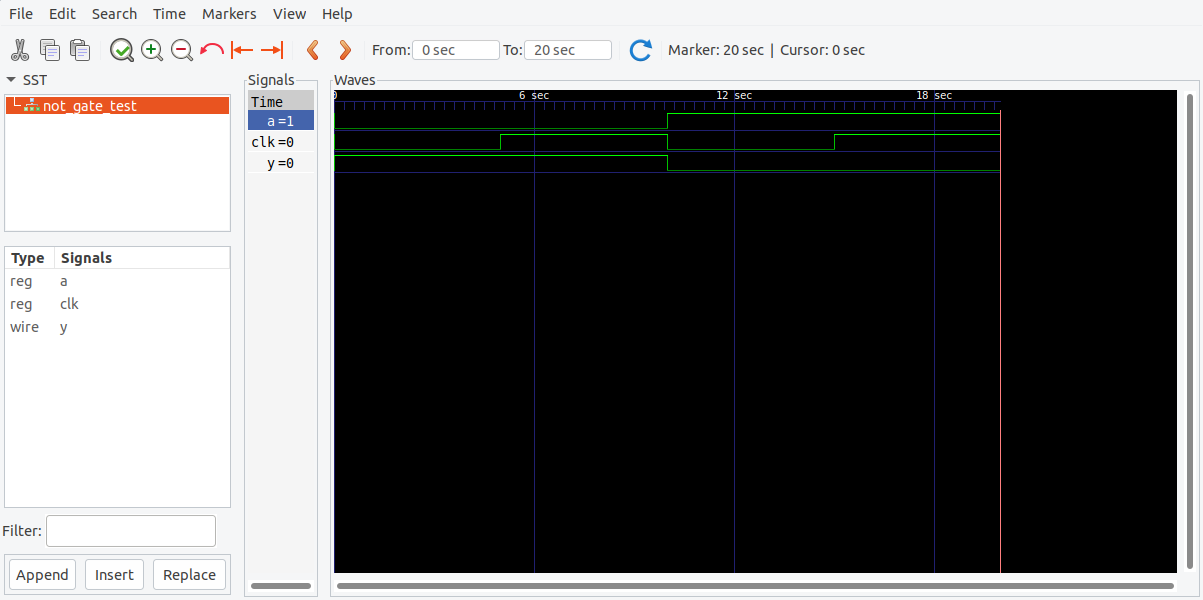
\includegraphics[width=1.0\textwidth]{not_gate_wf}
	\caption{Not Circuit Waveform}
	\label{fig: not_gate_wf}
\end{figure}

Here, both a and b are initialized to 0, so the output of the module, y, is 1 for the first 10 nanoseconds. Input a is then changed to 1 for the second 10 nanoseconds, then b is changed to 1 for the third. Finally, a is changed to 0 for the last 10 nanoseconds, For the last 30 nanoseconds, the output is always 0. This shows that for a Not Circuit, the output is always the opposite of the input, so if a is on, the output is 0, and it a is off, the output is 1. %\pagebreak
	\section{Nor Circuit}

The waveform for the Nor Circuit is shown below:
\begin{figure}[h]
	\centering
	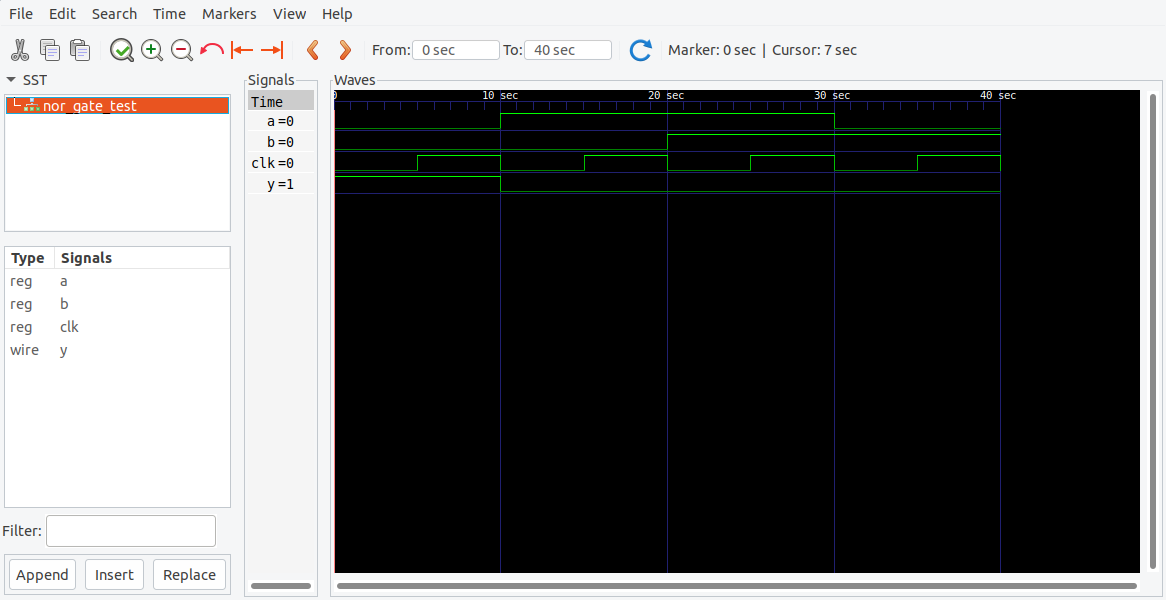
\includegraphics[width=1.10\textwidth]{nor_gate_wf}
	\caption{Nor Circuit Waveform}
	\label{fig: nor_gate_wf}
\end{figure}

Here, inputs a and b are both initialized to 0, which outputs 1, then a is changed to 0 for the second 10 nanoseconds and outputs 0. For the third 10 nanoseconds b is also set to 1, then a is changed back to 0 for the last 10 nanoseconds, which both of which output 0 again. This shows that for a Nor Circuit, the only time the output is 1 is when both a and b are off, otherwise the output is 0. \pagebreak
	\section{Nand Circuit}

The waveform for the Nand Circuit is shown below:

\begin{figure}[h]
	\centering
	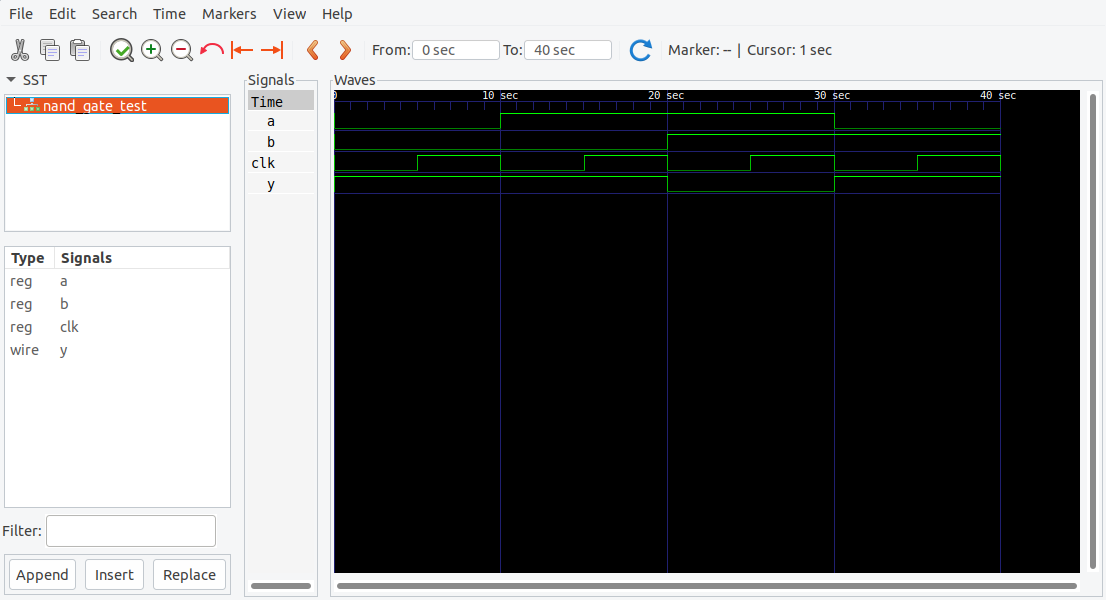
\includegraphics[width=1.0\textwidth]{nand_gate_wf}
	\caption{Nand Circuit Waveform}
	\label{fig: nand_gate_wf}
\end{figure}

Here, inputs a and b are both initialized to 0, then a is changed to 1 for the second 10 nanoseconds, both of which output 1. For the third 10 nanoseconds b is set to 1 and outputs 0, and finally a is changed back to 0 for the last 10 nanoseconds, which outputs 1. This shows that for a Nand Circuit, the only time that the output is 0 is when both inputs a and b are on, otherwise the output is 1.\pagebreak

\section{4-bit Shift}
The waveform for the 4-bit shift is shown below:

\begin{figure}[h]
	\centering
	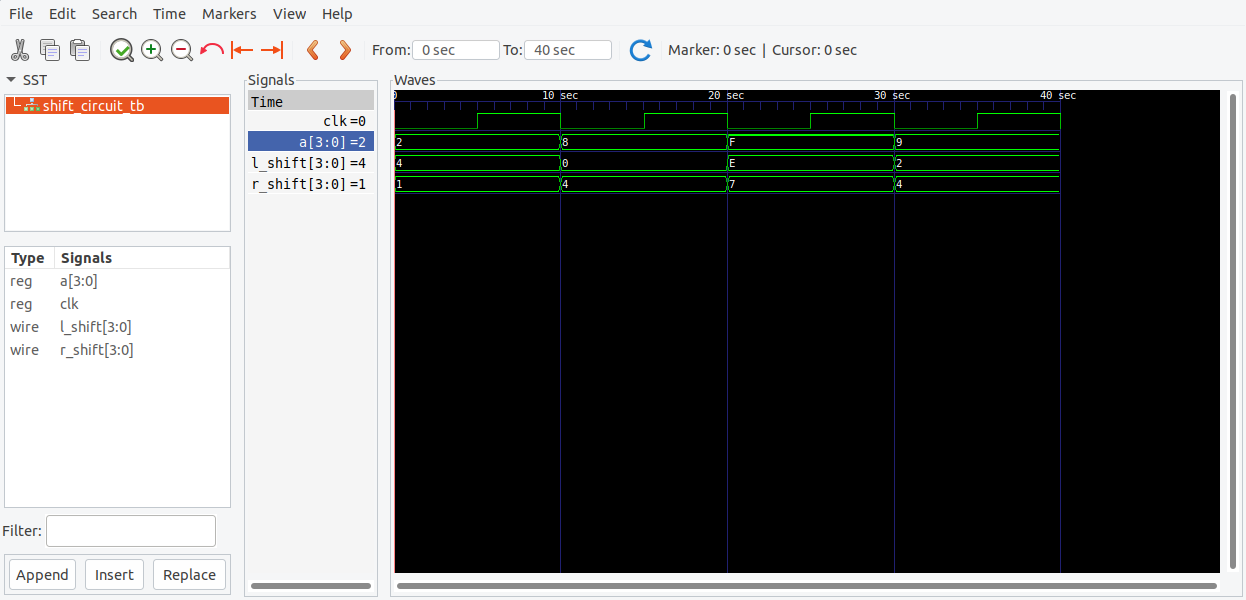
\includegraphics[width=1.10\textwidth]{shift_circuit_wf}
	\caption{Shift Circuit Waveform}
	\label{fig: shift_circuit_wf}
\end{figure}

Here, the input starts at 2 for the first 10 nanoseconds which outputs 4 for the left shit and 1 for the right shift, then moves to 8 for the second 10 nanoseconds, which outputs 0 for the left shift and 4 for the right shift. The third 10 nanoseconds has an input of F and a left shift output of E and a right shift output of 7. Finally, the input is 9 for the last 10 nanoseconds and outputs 2 for the left shift and 4 for the right shift.  \pagebreak

\chapter{conclusion}

	Given the requirements for this first project status report, I believe our group got the correct results. The code, test benches, and waveforms for the Not, Nor, Nand, and 4-bit Shift circuits seem to follow the truth tables for their corresponding logical and bitwise operations and inputs, so it stands to reason that they are correct and out project is successful so far. There was some difficulty in the beginning stages of the project mostly with getting all of the tools set up property and understanding how the Verilog syntax and compilation and waveform generation works. I know that Sam had some initial difficulty setting up his Ubuntu environment because he uses an apple laptop that has an 64-bit ARM processor that is fairly new, so finding a version of Ubuntu and VM software compatible with his hardware took a little bit of time. Once the environments were set up, the only real difficulty was understanding how the Verilog syntax works and how the compiled Verilog code works with GTK Wave to generate the waveforms we needed. The actual operations themselves were straightforward, so once we understood how to accomplish what the project is requiring we were able to get it done. 	
\end{document}
	